\scanpage{28}
Soit d'autre part
\[
\deleted{\unsure{A}}\ \mathbb A^{\unsure{'|\{}}(T)=
\left\{(t,\unsure{\pi|\Pi|\gamma},\bar a)\,\middle|\,
\begin{aligned}
&t\in T\\[-2pt]
&\pi\in\mathrm{Pol}(T\setminus\{t\})\\
&\bar a\in\mathrm{Ar}(\pi)/\mathrm{antipod}
\end{aligned}\right\}
\]
\inserted{$={}$Ens des $2$ diagonales du carré dual}

On voit que le cardinal de $\mathbb A'(T)$ est $5\cdot\frac12(4-1)!\cdot2=30$ \deleted{\unsure{$\times2=60$}}. Mais si $\alpha\in\mathbb A(T)$, $\alpha$ détermine une bijection
\[
T\simeq\{t\}\amalg a\times\varphi\qquad
(\text{où }\varphi=\mathrm{Ar}(\pi)\setminusa)
\]
d'où une orientation de $T$. Ainsi $\mathbb A(T)$ se décompose en $2$ paquets de $15$ éléments, associés aux deux orientations \inserted{$\unsure{\bar\omega|\varpi},-\bar\omega$} de $T$; on voit tout de suite que, sur chacun, telle $\mathbb A^+(T,\bar\omega)$, le groupe alterné $\mathrm{Alt}_T$ opère transitivemt. Ceci posé, on a une application canonique
\[
 A/\underline a\longrightarrow\mathbb A^+(T,\bar\omega),
\]
\inserted{compatible avec $G=\mathrm{Aut}(\Pi)$} et on voit comme précédemmt qu'elle est surjective, donc bijective.

Enfin, \unsure{on} a une application canonique
\[
 F/\underline a\longrightarrow\unsure{\mathscr P|\mathfrak P}_2(T)
\]
\figure{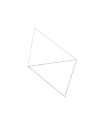
\begin{tikzpicture}[scale=.65,gray!45]
\draw[very thin] (0,0)--(.95,.13)--(.72,-.59)--cycle;
\draw[very thin,gray!25] (0,0)--(.13,.75)--(.95,.13);
\end{tikzpicture}}
compatible aux op. de $G$, donc (comme $\mathrm{Alt}_T$ est transitif sur $\mathscr P_2(T)$) surjective donc bijective.
% archive sheet number: 27
